%\begin{sidewaysfigure}
%  \begin{center}
%  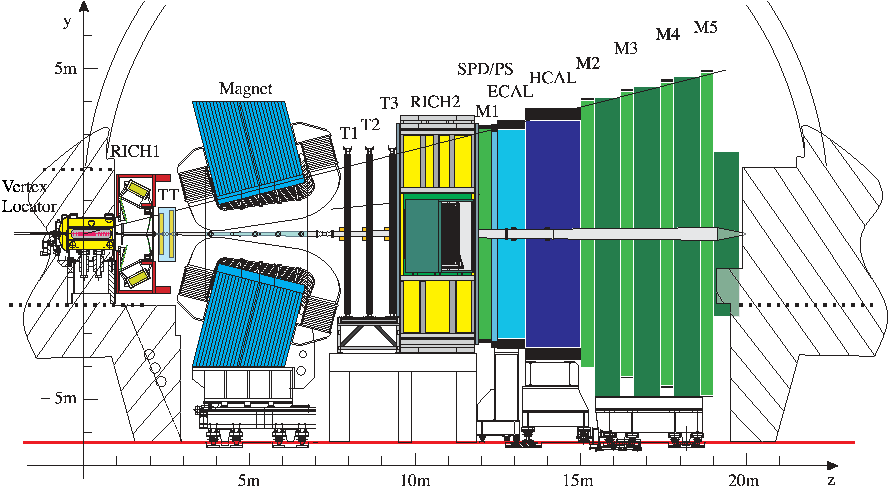
\includegraphics[width=0.8\textheight]{lhcb-detector-cross-section}
%  \caption[Cross-section view of \LHCb, cut in the non-bending $y$--$z$ plane]%
%    {Cross-section view of \LHCb, cut in the non-bending $y$--$z$ plane.}
%  \label{fig:LHCbCrossSection}
%  \end{center}
%\end{sidewaysfigure}



\chapter{The T2K Experiment}
\label{chap:T2KExperiment}


\section{Accelerator complex}
\label{sec:AcceleratorComplex}
These are words

\subsection{Proton Accelerators}
\label{subsec:ProtonAccelerators}
Stuff about the accelerator

\subsection{Neutrino beamline}
\label{subsec:NeutrinoBeamline}
Stuff about the beamline

\section{Near detector complex}
\label{sec:NearDetectorComplex}
Stuff about comples

\subsection{Multi-Pixel Photon Counter}
\label{subsec:MPPC}
MPPCs

\subsection{INGRID}
\label{subsec:INGRID}
Stuff about INGRID

\subsection{ND280}
\label{subsec:ND280}
ND280 time

\subsubsection{The fine grain detectors}
\label{subsubsec:FGD}
FGDS

\subsubsection{The time projection chambers}
\label{subsubsec:TPC}
TPCs

\subsubsection{The $\pi^0$ detector}
\label{subsubsec:pi0detector}
Here is ref for \ref{subsubsec:TPC}
pi0

\subsubsection{The electromagnetic calorimeters}
\label{subsubsec:ecal}
The beasts

\subsubsection{The side muon range detector}
\label{subsubsec:smrd}
Why bother?

\subsection{The far detector}
I mean SK


